\section{GTAC listening room modelling}
In the GTAC listening room there is a 96-loudspeaker array distributed as an irregular octagon in the horizontal plane (\autoref{GTAClab}), $1.65 \si{m}$ above the floor, with a separation between loudspeakers of $\secondarySourceSeparation = 0.18 \si{m}$. 

\begin{figure}
	\centering
	\begin{subfigure}[c]{0.55\textwidth}
		\centering
		\includegraphics[width=0.9\textwidth]{./Img/GTAClabPhoto.pdf}
		\caption{Picture \cite{Czy2011}}
		\label{GTAClabPhoto}
	\end{subfigure}
	\begin{subfigure}[c]{0.35\textwidth}
		\centering
		\reflectbox{\rotatebox[origin=c]{180}{
			\includegraphics[width=0.9\textwidth]{./Img/WFSarraySchemeReport.pdf}
	}}
		\caption[WFS array distribution]{Schematic of the loudspeaker array distribution}
		\label{WFSdistribution}
	\end{subfigure}
	\caption{GTAC listening room}
	\label{GTAClab}
\end{figure}

Many variables have an impact on the acoustic field generated by the loudspeakers: frequency dependent directivity of each individual loudspeaker, complex near-field radiation characteristics, non-linearities, reverberation of the chamber, diffraction, reflections on the floor (which is not recovered with absorbing material as the walls), etc. However, if we assume a simple model where the listening room is perfectly configured to emulate free-space conditions, and every loudspeaker is identical to the rest and behaves as an ideal monopole, then the similarities with the scenario presented by WFS theory become clear.

Under ideal conditions, the octagon can be interpreted as the closed curve of secondary sources $\sectionTheo$ discretized with a step of $\secondarySourceSeparation = 0.18 \si{m}$, so the aliasing frequency for a speed of sound $c = 340 \si{m/s}$ is $f_\mathit{alias} = 944.44\si{Hz}$.  As we only count with monopole sources (loudspeakers with dipole characteristics are more difficult and expensive to manufacture), we should use the Rayleigh 2.5D I integral (\autoref{RayleighI2.5}), but $\sectionTheo$ should be an infinite line and not an octagon. Of course, an infinite array is not realizable in practice, so at some point we must truncate the array anyway. On the other hand, when dealing with a bent array, the amplitude factor $g = \sqrt{\frac{d}{d + \abs{\PosTheo[primarySource][z]}}}$ that was calculated when $\sectionTheo$ was a straight line might not be the best option any more.

The actual loudspeaker feeding signals that were used, were calculated applying formulas that were provided by the professors and are particularized for the specific geometry of the GTAC array. Specifically, they follow the Rayleigh 2.5D I Integral form (\autoref{RayleighI2.5wfs}), where the amplitude factor $g$ is optimized for the middle line that divides the octagon in two equal halves:
\begin{equation}
\begin{aligned}
g &= 
\begin{cases}
\sqrt{\frac{d}{\distLinePrimSource + d}} & \normPrimaryPropAngle \leq 90^\circ \\
0 & \normPrimaryPropAngle > 90^\circ
\end{cases}
\\
d &= \frac{1.44}{2} + 1.44 \cos\left( \frac{\pi}{4} \right),
\end{aligned}
\label{amplitFactorGTAC}
\end{equation}
where $\normPrimaryPropAngle$ and $\distLinePrimSource$ are represented in
\autoref{figAngleCondition}. Other $g$ could have been used, although different variations were tested and the general trend of results didn't change.

For simplification purposes, from now on it will be assumed that primary sources are monopoles.

\section{Introduction to simulations}
Traditionally, WFS has been used, not to cancel noise, but as a spatial audio reproduction system that competes with existing stereophonic systems as Dolby Surround. The main focus has been, then, not in replicating accurately a field, but in generating the subjective impression of natural hearing, this is, of sound heard from various directions. So, the evaluation of performance has been usually guided by the ability of subjects to localize virtual sound sources and other subjective measures.

Since human hearing has limitations, there are objective sound characteristics that it cannot perceive. We can take advantage of this, and use compression, downsampling and other techniques (common in mp3 and other compression formats) that lower the requirements of the system without worsening the subjective perception. One thing that humans cannot distinguish is constant phase shift with frequency. So, when implementing WFS, the term $\sqrt{j}$ can be omitted (as done in the real implementations in \cite{Verheijen} and \cite{Vogel}) since it would require the implementation of a FIR filter that would not add anything to the experience of the audience. Depending on the requirements of the system, the frequency dependent coefficient $\sqrt{k}$ can also be omitted, with the disadvantage that it would produce coloration of the sound (\cite{Vogel}).

Without both filters, the signal of a given loudspeaker can be calculated by just applying a delay to the virtual source signal and multiplying it by a scalar.
\begin{gather}
\signal[wfs][frequency](f) = \signal[nsVirt][frequency](f) \cos\normPrimaryPropAngleSection \frac{e^{-jk\distLinePrimSource}}{\sqrt{\distLinePrimSource}} g
\\
\signal[wfs][time](t) = \signal[nsVirt][time](t) \frac{g \cos\normPrimaryPropAngleSection}{\sqrt{\distLinePrimSource}}
\ast\delta(t - \distLinePrimSource/c),
\label{wfsSignalTime}
\end{gather}
where $\ast$ is the convolution operator, and $\signal[nsVirt][time](t) = -\signal[ns][time](t)$ is the signal transmitted by the primary source, now called virtual noise source because it is the same as the signal transmitted by the noise source multiplied by $-1$.
\begin{figure}
	\centering
	\def\svgwidth{0.4\columnwidth}
	\graphicspath{{Img/}}
	\input{Img/WFSParameters.pdf_tex}
	\caption[WFS calculation parameters]{WFS calculation parameters}
	\label{figAngleCondition}
\end{figure}

This is the first approach we used in simulations. As an example, let's consider the situation in \autoref{oneReceiverOneNSScheme}. A sinusoidal signals of frequency $440 \si{Hz}$ is transmitted by the noise source in free-space conditions. All loudspeakers transmit signals according to \autoref{wfsSignalTime}. The signal received at the centre of the octagon is shown in \autoref{oneReceiverPureDeltaReceived}. Ideally, the signal received from the noise source $\Field[ns][time]$ and the loudspeaker array $\Field[wfs][time]$ should be opposite, but it is clear they are not.

\begin{figure}
	\centering
	\begin{subfigure}[c]{0.45\textwidth}
	\centering
	\reflectbox{\rotatebox[origin=c]{180}{
			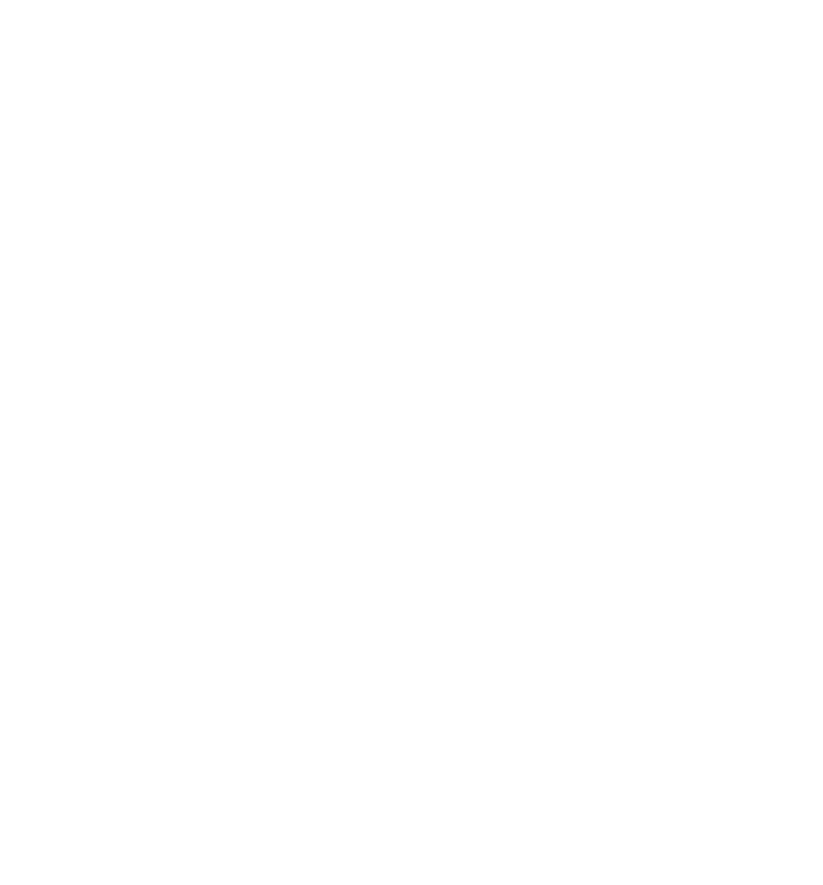
\includegraphics[width=\columnwidth]{./Img/Experiment11_scheme_oneReceiver.pdf}
	}}
	\caption[Scheme of basic scenario]{Scheme of basic scenario with one noise source and one point of measure}
	\label{oneReceiverOneNSScheme}
	\end{subfigure}
	\begin{subfigure}[c]{0.45\textwidth}
		\centering
		%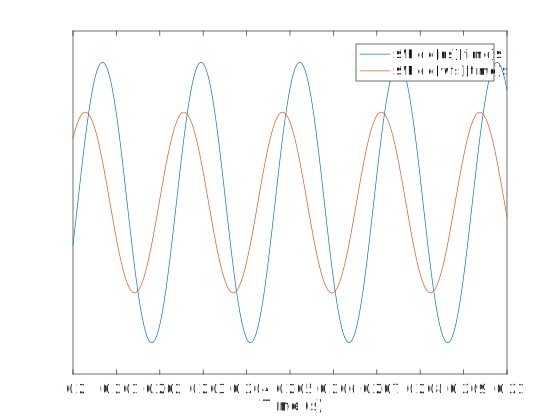
\includegraphics[width=\columnwidth]{Img/Experiment11_exampleNoFreqCorr.eps}		
		\def\svgwidth{1.2\columnwidth}
		\graphicspath{{Img/}}
			{\fontsize{5}{12}\selectfont
		\input{Img/Experiment11_exampleNoFreqCorr.pdf_tex}
	}
		\caption{Signal measured}
		\label{oneReceiverPureDeltaReceived}
	\end{subfigure}
	\caption{Simulation in simple scenario with one noise source and one point of measure}
\end{figure}

In order to quantify the performance, we will use the concept of gain $\gain$. It is a frequency dependent parameter, defined as the power of the received signal at a given point divided by the power of the signal received exclusively from the noise source. %The inverse of the gain is the cancellation $\cancellation$. We will express them usually in dB:
\begin{gather}
\gain(f) = 10\log{\left\lvert\frac{\Field[wfs][frequency](f) + \Field[ns][frequency](f)}{\Field[ns][frequency](f)}\right\rvert^2}\quad\si{dB},%\\
%\cancellation(f) = -\gain(f),
\end{gather}
where $\Field[ns][frequency](f)$ and $\Field[wfs][frequency](f)$ are the frequency components at $f \si{Hz}$ of the signals received from the noise source and loudspeaker array respectively. From now on, the frequency dependence will not be explicitly indicated: $\gain = \gain(f)$, $\Field[ns][frequency] = \Field[ns][frequency](f)$, etc. Sometimes we will use the terms cancellation or attenuation, referring to the inverse of the gain. For example, saying "cancellation levels should be higher than $8 \si{dB}$" is equivalent to saying "gain levels should be lower than $-8 \si{dB}$". Depending on the context, one or the other term will be used.
The maximum cancellation (or minimum gain) will happen when $\Field[ns][frequency] = -\Field[wfs][frequency]$.

Another useful parameter is what I call correction factor $\correctionFactor$. It is conceived as the complex number by which loudspeakers signals $\signal[wfs][frequency]$ should be multiplied in order to achieve maximum cancellation:
\begin{equation}
\correctionFactor = -\frac{\Field[ns][frequency]}{\Field[wfs][frequency]}.
\end{equation}

In the previous case, the gain and corrections factors are $\gain = 3.6\si{dB}$ and $\correctionFactor = 1.1 e^{j40.3/360}$.

Since the aim of WFS is achieving cancellation over an wide area, it is reasonable to measure the field not in just one location, but in a grid of points, and the cancellation will vary from one to another. In that case, it is convenient come up with some way of describing the overall performance with just one value that takes in account the field at every point of measure.
The concept of average gain, $\averageGain$, can be used. Assuming there are $\numMeasPoints$ points of measure:
\begin{equation}
	\averageGain = 10\log\left(\frac{1}{\numMeasPoints} \sum_{m=1}^\numMeasPoints \abs{\frac{\Field[wfs][frequency][scalar][m] + \Field[ns][frequency][scalar][m]}{\Field[ns][frequency][scalar][m]}}^2\right) \quad \si{dB},
\end{equation}
where $\Field[wfs][frequency][scalar][m]$ and $\Field[ns][frequency][scalar][m]$ are the field produced at the $m$-th point of measure by the loudspeaker array and the noise source respectively.

\begin{shownto}{publicGlobal}
	The concept of global gain can also be used, defined as the overall total power divided by the overall measured power with the loudspeakers turned off:
	\begin{gather}
		\globalGain = 10 \log \left[\frac{\sum_{m=1}^\numMeasPoints \abs{\Field[ns][frequency][scalar][m] + \Field[wfs][frequency][scalar][m]}^2}{\sum_{m=1}^\numMeasPoints \abs{\Field[ns][frequency][scalar][m]}^2}\right] \quad \si{dB}
		\\
		\globalCancellation = -\globalGain
	\end{gather}
\end{shownto}

In the same way, the correction factor has a global equivalent, the global correction factor $\globalCorrectionFactorAverGain$, defined as the number that must be multiplied by the loudspeaker signals $\signal[wfs][frequency]$ in order to minimize the average gain.
\begin{equation}
\globalCorrectionFactorAverGain(f) = \argmin_{\psi} \sum_{m=1}^\numMeasPoints \abs{\frac{\psi \Field[wfs][frequency][scalar][m] + \Field[ns][frequency][scalar][m]}{\Field[ns][frequency][scalar][m]}}^2 =
-\frac{\left(\sum_{m=1}^\numMeasPoints \Field[wfs][frequency][scalar][m]/\Field[ns][frequency][scalar][m]\right)^*}{\sum_{m=1}^\numMeasPoints \abs{\Field[wfs][frequency][scalar][m]/\Field[ns][frequency][scalar][m]}^2},
\end{equation}
where $^*$ is the complex conjugate symbol.

\begin{shownto}{publicGlobal,private}	
A variant of the global correction factor, $\globalCorrectionFactor$, can also be used. It is the same as $\globalCorrectionFactorAverGain$, but designed to minimize the overall measured power instead of the average gain.
% It is defined as the number that must be multiplied by the loudspeaker signals $\signal[wfs][frequency]$ in order to minimize the overall measured power.
	\begin{equation}
	\globalCorrectionFactor = \argmin_{\psi} \norm{\psi \Field[wfs][frequency][vector] + \Field[ns][frequency][vector]}^2 = -\frac{\scalarProd{\Field[wfs][frequency][vector]^*}{\Field[ns][frequency][vector]}}{\norm{\Field[wfs][frequency][vector]}^2}
	\end{equation}
	where $\Field[wfs][frequency][vector] = [\Field[wfs][frequency][scalar][1],...,\Field[wfs][frequency][scalar][\numMeasPoints]]^T$ and $\Field[ns][frequency][vector] = [\Field[ns][frequency][scalar][1],...,\Field[ns][frequency][scalar][\numMeasPoints]]^T$.
\end{shownto}

So, instead of one point, now let's see what happens at a grid of points (\autoref{MultipleReceiverOneNSCanc}). It seems cancellation is bad at all of them. \showto{publicGlobal}{The global cancellation value is $\globalCancellation = 2.37 dB$.} The average gain value is $\averageGain = 2.55 \si{dB}$.

\begin{figure}
	\centering			\includegraphics[height=0.3\textheight]{./Img/Experiment11_multipleReceiverAtten2Dmap.eps}
	\caption[Gain 2D map]{Gain 2D map in dB}
	\label{MultipleReceiverOneNSCanc}
\end{figure}

It might be that the bad results have to do with the location of the noise source. Let's then see what happens for different positions as shown in \autoref{MultRecMultNSscheme}. Instead of just showing the 2D map of cancellations for each noise source positions, it will be more convenient for further analysis to visualize it as a histogram of 
\showto{publicGlobal}{global gain values (\autoref{histogramDifNSNoFreqCorrGlobGain}) or a histogram of}
average gain values (\autoref{histogramDifNSNoFreqCorrAverGain}). The values express probability: number of occurrences in a given gain interval divided by the total number of occurrences.

\begin{figure}
	\centering
	\begin{subfigure}[b]{0.49\textwidth}
	\centering
	\reflectbox{\rotatebox[origin=c]{180}{
			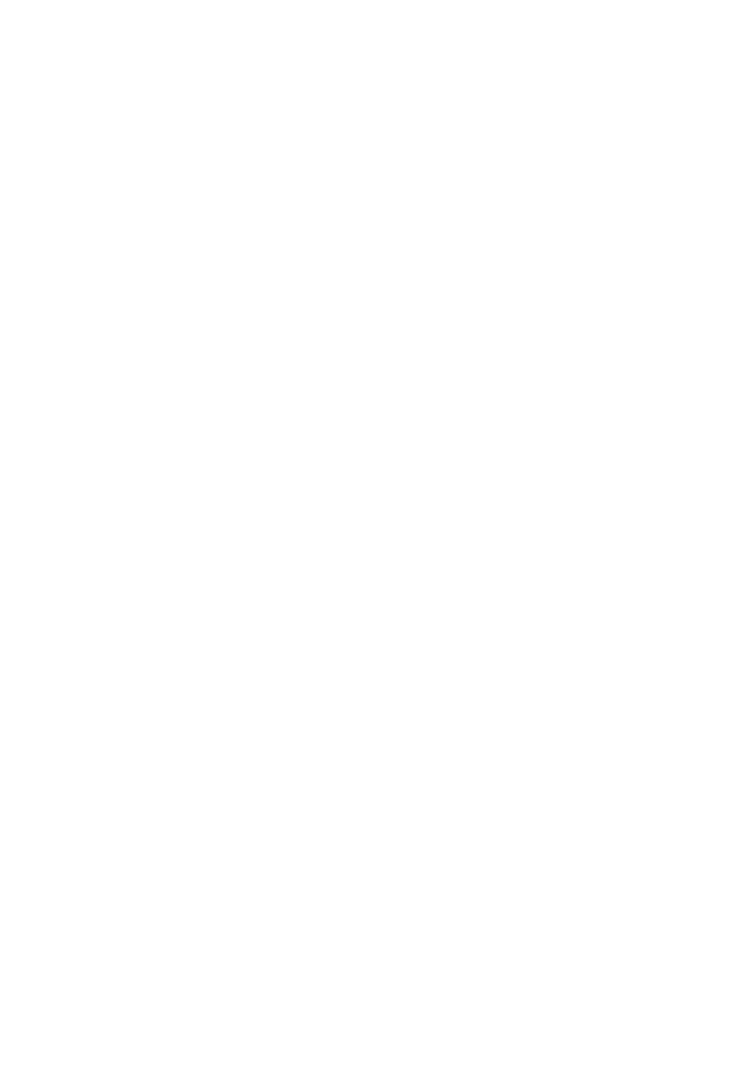
\includegraphics[height=0.3\textheight]{./Img/Experiment11_scheme_multipleReceiverMultipleNS.pdf}
	}}
	\caption[Scheme of multiple points of measure and multiple noise source positions]{Scheme of multiple points of measure and multiple noise source positions}
	\label{MultRecMultNSscheme}
	\end{subfigure}
	\showto{publicGlobal}{
	\begin{subfigure}[b]{0.49\textwidth}
		\centering
		\includegraphics[height=0.3\textheight]{./Img/Experiment11_attenGlobDifNSNoFreqCor.eps}
		\caption{Histogram of global gains}
		\label{histogramDifNSNoFreqCorrGlobGain}
	\end{subfigure}
	}
	\begin{subfigure}[b]{0.49\textwidth}
		\centering
		\includegraphics[height=0.3\textheight]{./Img/Experiment11_gainAverDifNSNoFreqCor.eps}
		\caption{Histogram of average gains}
		\label{histogramDifNSNoFreqCorrAverGain}
	\end{subfigure}
	\caption{Multiple positions of the noise source}
\end{figure}

However, all this has been tested just at one frequency. Maybe, the behaviour for the rest of frequencies is different. To check it out, we will make the noise source transmit a chirp signal from $20 \si{Hz}$ to $940 \si{Hz}$ (close to the aliasing spatial frequency) and then calculate the FFT\showto{private}{(for more information on how the simulations are carried out, consult appendix \autoref{appendixSimulation})}. The average gain for one noise source position is shown in \autoref{averGainOneNSchirp}.
\showto{private}{The global gain for one noise source position is shown in \autoref{globCancOneNSchirp}.}
It is obvious that the values are bad over the whole bandwidth.

\begin{figure}[h]
	\centering
	\includegraphics[width=0.4\textwidth]{./Img/Experiment11_gainAverOneNSChirp.eps}
	\caption{Average gain for the whole bandwidth and a given noise source position}
	\label{averGainOneNSchirp}
\end{figure}

\showto{publicGlobal,private}{
\begin{figure}[h]
	\centering
	\includegraphics[width=0.4\textwidth]{./Img/Experiment11_globalCancOneNSChirp.eps}
	\caption{Global gain for the whole bandwidth and a given noise source position}
	\label{globCancOneNSchirp}
\end{figure}
}

In order to understand what is happening for the whole bandwidth and multiple source position in just one snapshot, consider \autoref{histogram3D}. It is a probability histogram of global gains, similar to \autoref{histogramDifNSNoFreqCorrAverGain}, but seen in 3D, and each bar has been coloured according to the height. If we look at it from above (\autoref{histogram3Dabove}), we will not appreciate the heigh, but the colour will be enough.
That histogram is particularized for just one frequency ($440\si{Hz}$). If, for each frequency, we generate a similar coloured histogram and stack them next to each other, we can form an image as \autoref{histogramGainAverDifNS}. %where the x axis is the frequency, the y axis is the gain value, and the colour is the number of occurrences in that interval divided by the total number of occurrences for that frequency interval;
Each coloured rectangle is bounded horizontally ($x$ axis) by two frequency values and vertically ($y$ axis) by two gain values. The colour indicates the number of occurrences in that frequency and gain intervals divided by the total number of occurrences for that frequency interval;
in other words, each column is an independent probability histogram. The histogram tells us that cancellation is bad at all frequencies, for every position of the noise source.

\begin{figure}[h]
	\centering
	\begin{subfigure}[b]{0.49\textwidth}
	\centering
	\includegraphics[width=0.8\textwidth]{./Img/Experiment11_gainAverDifNSchirp3Dhist.eps}
	\caption{Example of average gain histogram in 3D}
	\label{histogram3D}
	\end{subfigure}
	\begin{subfigure}[b]{0.49\textwidth}
		\centering
		\includegraphics[width=0.8\textwidth]{./Img/Experiment11_gainAverDifNSchirp3DhistAbove.eps}
		\caption{Example of average gain histogram in 3D seen from above}
		\label{histogram3Dabove}
	\end{subfigure}
	\begin{subfigure}[b]{0.49\textwidth}
		\centering	\includegraphics[width=0.8\textwidth]{./Img/Experiment11_DifNSchirpGainAver.eps}
		\caption{Completed average gain histogram}
		\label{histogramGainAverDifNS}
	\end{subfigure}
	\showto{publicGlobal}{
	\begin{subfigure}[b]{0.49\textwidth}
		\centering	\includegraphics[width=0.8\textwidth]{./Img/Experiment11_DifNSchirpGlobAtten.eps}
		\caption{Completed global gain histogram}
		\label{histogramGlobAttenDifNS}
	\end{subfigure}
	}
\caption{Frequency dependent histogram of gain, step by step}
\end{figure}

What is happening? The answer can be found if we represent the global correction factor $\globalCorrectionFactorAverGain$ (\autoref{GlobalCorrFactAverGain}) \showto{publicGlobal}{and $\globalCorrectionFactor$ (\autoref{GlobalCorrFact})}. We can see that, even when there is some variance between the values for different noise source positions, the overall tendency follows the theoretical expression $\sqrt{jk/2\pi}$ that was omitted for being considered unnecessary. This result suggests that it is, indeed, necessary.

\begin{figure}[h]
	\begin{subfigure}[b]{0.49\textwidth}
		\centering
		\includegraphics[width=0.8\textwidth]{./Img/Experiment11_DifNSchirpGlobCorrAverGainFactAbs.eps}
		\caption{$\abs{\globalCorrectionFactorAverGain}$}
		\label{GlobalCorrFactAbsAverGain}
	\end{subfigure}
	\begin{subfigure}[b]{0.49\textwidth}
		\centering
		\includegraphics[width=0.8\textwidth]{./Img/Experiment11_DifNSchirpGlobCorrAverGainFactPhase.eps}
		\caption{$\angle{\globalCorrectionFactorAverGain}$}
		\label{GlobalCorrFactPhaseAverGain}
	\end{subfigure}
\caption{Global correction factor $\globalCorrectionFactorAverGain$}
\label{GlobalCorrFactAverGain}
\end{figure}

\showto{publicGlobal}{
\begin{figure}[h]
	\begin{subfigure}[b]{0.49\textwidth}
		\centering
		\includegraphics[width=0.8\textwidth]{./Img/Experiment11_DifNSchirpGlobCorrFactAbs.eps}
		\caption{$\abs{\globalCorrectionFactor}$}
		\label{GlobalCorrFactAbs}
	\end{subfigure}
	\begin{subfigure}[b]{0.49\textwidth}
		\centering
		\includegraphics[width=0.8\textwidth]{./Img/Experiment11_DifNSchirpGlobCorrFactPhase.eps}
		\caption{$\angle{\globalCorrectionFactor}$}
		\label{GlobalCorrFactPhase}
	\end{subfigure}
	\caption{Global correction factor $\globalCorrectionFactor$}
	\label{GlobalCorrFact}
\end{figure}
}

The reason for this is that, even though that term is expendable when generating wave fields that are going to be heard by humans, it is required when the aim is to interference destructively with another existing wave field. For example, for a noise field $\Field[ns][frequency] = 1$, the secondary source field should be $\Field[wfs][frequency] = -1$ for perfect cancellation $\attenuation = -\infty \si{dB}$. But if the phase is shifted $-\pi/4$ ($1/\sqrt{j} = e^{-j\pi/4}$), the amplitude of the field is $|\Field[ns][frequency] + \Field[wfs][frequency]| = |1 - e^{-j\pi/4}| = 0.77$, which corresponds to a cancellation of $\cancellation = 2.32\si{dB}$. Amplitude variations of course also worsen the cancellation levels. So, the term $\sqrt{jk/2\pi}$ might irrelevant when for the human ear when listening to a signal, but are of vital importance if we are going to make a cancelling wave physically interfere with another. We can't get away with just ignoring it.

In conclusion, %before the delay and amplitude modification, the noise source signal must be filtered by a "prefilter" with response $\sqrt{jk/2\pi}$ if the intention is to perform active cancellation of noise.
a $\sqrt{jk/2\pi}$ filter must be implemented in WFS when the intention is to perform active cancellation of noise.
This is not a major problem in terms of computational efficiency because this filtering is common to all secondary loudspeakers, so it can be carried out just once on the primary source signal, and then apply the delay and amplitude modification corresponding to each secondary source independently. That is why we talk about "prefiltering".
Nevertheless, it presents the problem that, theoretically, the prefilter has an anticausal response, but it must be implemented as a FIR digital filter, so inevitably it will introduce some amount of delay that must be compensated \cite{Lapini2018}. That sets a constraint on how close the noise source can be to the loudspeaker array, as we will see in next section.

\section{Compromise between frequency filter length and accuracy}

\begin{shownto}{private}
	%Consultar \cite{FrankSchutz2015}
\end{shownto}

In previous section we've concluded that, in order to produce cancellation inside the area enclosed by the loudspeaker array, a filter with a frequency response $\sqrt{jk/2\pi} = \sqrt{jf/c}$ must be implemented, traditionally in the form of a FIR digital filter. This has a drawback, and it is that the ideal theoretical filter is anticausal. This means that, in order to calculate the output signal $y$ at a time $t$, it needs to use input values that come after that time: $y(t)$ depends on $x(t+\Delta t)$, being $\Delta t > 0$. This is exactly like knowing the future. Mathematically speaking, that can make sense, and in simulations it is not a limitation either since we know exactly what the noise source signal is going to be.
But in real-time systems it is, obviously, impossible to implement.

However, there is a nuance that can allow us to implement this filter in real-time. Let's complete \autoref{wfsSignalTime} with the new filter:
\begin{equation}
\begin{aligned}
\signal[wfs][time](t) &= \signal[nsVirt][time](t) \frac{g \cos\normPrimaryPropAngleSection}{\sqrt{\distLinePrimSource}}
\ast\delta(t - \distLinePrimSource/c)\ast \freqFilter(t) = \signal[nsVirt][time](t) \frac{g \cos\normPrimaryPropAngleSection}{\sqrt{\distLinePrimSource}}
\ast \freqFilter(t - \distLinePrimSource/c)\\
\freqFilter(t) &= \FourierTransform{\sqrt{\frac{jk}{2\pi}}}[inverse].
\end{aligned}
\label{rayleigh2_5Dsignal}
\end{equation}

When we say that $\freqFilter(t)$ is anticausal, it is the same as saying that there are negative values of $t$ for which $\freqFilter(t) \neq 0$. As long at this does not change, the practical implementation of this filter will not be possible. Nonetheless, let's notice that the loudspeaker signal $\signal[wfs][time](t)$ does not depend directly on $\signal[nsVirt][time](t)$ filtered by $\freqFilter(t)$, but on a delayed version of it: $\freqFilter(t - \distLinePrimSource/c)$.

If the filter impulse response $\freqFilter(t)$ was limited in time ($\freqFilter(t) = 0, t < -\tau_1$), then, although $\freqFilter(t)$ would be anticausal, $\freqFilter(t - \distLinePrimSource/c)$ will be causal as long as $\distLinePrimSource/c > \tau_1$. However, since the ideal $\freqFilter(t)$ has an infinite response, the only option left is to use an approximation ($\widetilde{\freqFilter}(t)$) that satisfies that $\widetilde{\freqFilter}(t) = 0$ for $t < -\tau_1$, where $\tau_1 < \distLinePrimSource/c$. The delayed filter $\widetilde{\freqFilter}(t - \distLinePrimSource/c)$ is causal, and hence could work in a real time system.

If, in addition, it has a finite duration, it would be implementable as a FIR digital filter. This means it must satisfy that $\freqFilter(t) = 0, t \notin [-\tau_1, \tau_2]$. However, as it works as an approximation, the smaller $\distLinePrimSource/c$ gets, the shorter the duration of the impulse response needs to be, and hence the worse the approximation and the accuracy of WFS will be. So, there is actually a trade-off between performance and the distance between the source and the closest loudspeaker $\distLinePrimSource$. The smaller the distance, the worse the performance. At a given sampling frequency, which is $44100 \si{Hz}$ in our simulations, the duration of the impulse response translates directly to number of coefficients of the digital filter.

We should differentiate between the filter that implements the magnitude of the frequency response $\freqFilter[time][magnitude] = \FourierTransform{\sqrt{f/c}}[inverse]$ and the one that implements the frequency independent phase shift $\freqFilter[time][phase] = \FourierTransform{\sqrt{j}}[inverse]$, because they present different requirements. The real implementations will be called $\widetilde{\freqFilter[time][magnitude]}$ and $\widetilde{\freqFilter[time][phase]}$ respectively.

A way of generating this filters is by using the analytical discrete impulse responses that were provided in \cite{FrankSchutz2015}[Equation 2.192 and 2.194] for the phase and magnitude filters respectively:
\begin{gather}
	{h_{mag}}[n] = \begin{cases}
		-\frac{S(\sqrt{2n})}{\sqrt{2\pi}n^{3/2}}, & n \neq 0 \\
		\frac{2}{3}\sqrt{\pi}, & n = 0
	\end{cases} \\
	{h_{pha}}[n] = \begin{cases}
		0, & \text{if $n$ is even and $n \neq 0$} \\
		\frac{-\sqrt{2}}{\pi n}, & \text{if $n$ is odd} \\
		\frac{1}{\sqrt{2}}, & n = 0
	\end{cases}
\end{gather}
where $S$ is the fresnel sine integral function (fresnels in Matlab).

The response of the magnitude filter $h_{mag}$ when the number of coefficients is infinite is:
\begin{equation}
H_{mag}(f) = \frac{2}{5}\sqrt{\frac{f}{f_s}}.
\end{equation}

As the ideal filter we want to get has a magnitude response $\sqrt{f/c}$ at a sampling frequency $f_s$, the magnitude filter must be scaled in order to fit our purposes:
\begin{equation}
\freqFilter[frequency][magnitude] = H_{mag}\frac{5}{2}\sqrt{\frac{f_s}{c}}. %\rightarrow \freqFilter[time][magnitude] = \frac{5}{2}\sqrt{\frac{f_s}{c}}h_{mag}
\end{equation}
Finally, we must choose a window function in order to make it finite.

Matlab also has its own internal functions to design FIR filters based on their frequency response and the number of coefficients, and in the case of these filters, it also returns symmetrical impulse responses ($\tau_1 = \tau_2 = \tau$). Using anyone of both ways (Matlab built-in function or analytical equations with rectangular window or Kaiser-Bessel window as proposed in \cite{FrankSchutz2015}), results are pretty similar. Using other window functions may improve filter response. Next simulations use the Matlab functions because, as they use optimization algorithms to find the most accurate response possible for a given number of coefficients, it is very likely that the generated filter it's close to the best possible configuration. But, as said before, results are actually pretty similar anyway.

We have plotted the histograms of gain for different lengths of the implementation of $\widetilde{\freqFilter[time][magnitude]}$ (\autoref{gainAverDifMagFilterLength}), keeping $\widetilde{\freqFilter[time][phase]}$ with a high enough length so it resembles the ideal case and does not produce any noticeable distortion. We can see that, below an order of $64$ (the order of a FIR filter is its length minus 1), the performance starts to get worse and worse. Above it, the improvement is not too noticeable.
\begin{shownto}{publicGlobal}
\begin{figure}[h]
	\centering
	\begin{subfigure}[b]{0.45\textwidth}
		\centering
		\includegraphics[width=\columnwidth]{../TFM/Img/Experiment12_globalAttenMagnOrder_8.eps}
		\caption{Order: $8$. $\tau = 0.091 \si{ms}$. ${\distLinePrimSource}_{min} = 3\si{cm}$}
	\end{subfigure}
	\begin{subfigure}[b]{0.45\textwidth}
		\centering
		\includegraphics[width=\columnwidth]{../TFM/Img/Experiment12_globalAttenMagnOrder_16.eps}
		\caption{Order: $16$. $\tau = 0.181 \si{ms}$. ${\distLinePrimSource}_{min} = 6\si{cm}$}
	\end{subfigure}
	\begin{subfigure}[b]{0.45\textwidth}
		\centering
		\includegraphics[width=\columnwidth]{../TFM/Img/Experiment12_globalAttenMagnOrder_32.eps}
		\caption{Order: $32$. $\tau = 0.363 \si{ms}$. ${\distLinePrimSource}_{min} = 12\si{cm}$}
	\end{subfigure}
	\begin{subfigure}[b]{0.45\textwidth}
		\centering
		\includegraphics[width=\columnwidth]{../TFM/Img/Experiment12_globalAttenMagnOrder_64.eps}
		\caption{Order: $64$. $\tau = 0.726 \si{ms}$. ${\distLinePrimSource}_{min} = 25\si{cm}$}
	\end{subfigure}
	
	\caption{Global gain for different lengths of $\freqFilter[time][magnitude]$}
	\label{globCancDifMagFilterLength}
\end{figure}
\end{shownto}
\begin{figure}[h]
	\centering
	\begin{subfigure}[b]{0.45\textwidth}
		\centering
		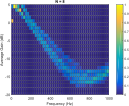
\includegraphics[width=\columnwidth]{../TFM/Img/Experiment12_globalGainAverMagnOrder_8.eps}
		\caption{Order: $8$. $\tau = 0.091 \si{ms}$. ${\distLinePrimSource}_{min} = 3\si{cm}$}
	\end{subfigure}
	\begin{subfigure}[b]{0.45\textwidth}
		\centering
		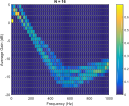
\includegraphics[width=\columnwidth]{../TFM/Img/Experiment12_globalGainAverMagnOrder_16.eps}
		\caption{Order: $16$. $\tau = 0.181 \si{ms}$. ${\distLinePrimSource}_{min} = 6\si{cm}$}
	\end{subfigure}
	\begin{subfigure}[b]{0.45\textwidth}
		\centering
		\includegraphics[width=\columnwidth]{../TFM/Img/Experiment12_globalGainAverMagnOrder_32.eps}
		\caption{Order: $32$. $\tau = 0.363 \si{ms}$. ${\distLinePrimSource}_{min} = 12\si{cm}$}
	\end{subfigure}
	\begin{subfigure}[b]{0.45\textwidth}
		\centering
		\includegraphics[width=\columnwidth]{../TFM/Img/Experiment12_globalGainAverMagnOrder_64.eps}
		\caption{Order: $64$. $\tau = 0.726 \si{ms}$. ${\distLinePrimSource}_{min} = 25\si{cm}$}
	\end{subfigure}
	
	\caption{Average gain for different lengths of $\freqFilter[time][magnitude]$}
	\label{gainAverDifMagFilterLength}
\end{figure}


We've done the same with $\freqFilter[time][phase] = \FourierTransform{\sqrt{j}}[inverse]$. In this case, a Hilbert filter must be implemented and, as we see in (\autoref{gainAverDifHilFilterLength}), its length has to be much bigger than with the magnitude filter length. It entails a more severe constraint. $\widetilde{\freqFilter[time][magnitude]}$ order is high enough so produced distortions are negligible. Orders of $4096$ and above get practically the same levels of attenuation, so it makes no sense to go beyond $4096$. However, such a long filter implies that the distance from the noise source to the closest loudspeaker should be at least $15.79 \si{m}$, a restriction that can not always be met.
\begin{shownto}{publicGlobal}
\begin{figure}[h]
	\centering
	\begin{subfigure}[b]{0.45\textwidth}
		\centering
		\includegraphics[width=\columnwidth]{../TFM/Img/Experiment12_globalAttenHilbOrder_512.eps}
		\caption{Order: $512$. $\tau = 5.8 \si{ms}$. ${\distLinePrimSource}_{min} = 1.97\si{m}$}
	\end{subfigure}
	\begin{subfigure}[b]{0.45\textwidth}
		\centering
		\includegraphics[width=\columnwidth]{../TFM/Img/Experiment12_globalAttenHilbOrder_1024.eps}
		\caption{Order: $1024$. $\tau = 11.6 \si{ms}$. ${\distLinePrimSource}_{min} = 3.95\si{m}$}
	\end{subfigure}
	\begin{subfigure}[b]{0.45\textwidth}
		\centering
		\includegraphics[width=\columnwidth]{../TFM/Img/Experiment12_globalAttenHilbOrder_2048.eps}
		\caption{Order: $2048$. $\tau = 23.2 \si{ms}$. ${\distLinePrimSource}_{min} = 7.89\si{m}$}
	\end{subfigure}
	\begin{subfigure}[b]{0.45\textwidth}
		\centering
		\includegraphics[width=\columnwidth]{../TFM/Img/Experiment12_globalAttenHilbOrder_4096.eps}
		\caption{Order: $4096$. $\tau = 46.4 \si{ms}$. ${\distLinePrimSource}_{min} = 15.79\si{m}$}
	\end{subfigure}
	
	\caption{Global gain for different lengths of $\freqFilter[time][phase]$}
	\label{globCancDifHilFilterLength}
\end{figure}
\end{shownto}

\begin{figure}[h]
	\centering
	\begin{subfigure}[b]{0.45\textwidth}
		\centering
		\includegraphics[width=\columnwidth]{../TFM/Img/Experiment12_gainAverHilbOrder_512.eps}
		\caption{Order: $512$. $\tau = 5.8 \si{ms}$. ${\distLinePrimSource}_{min} = 1.97\si{m}$}
	\end{subfigure}
	\begin{subfigure}[b]{0.45\textwidth}
		\centering
		\includegraphics[width=\columnwidth]{../TFM/Img/Experiment12_gainAverHilbOrder_1024.eps}
		\caption{Order: $1024$. $\tau = 11.6 \si{ms}$. ${\distLinePrimSource}_{min} = 3.95\si{m}$}
	\end{subfigure}
	\begin{subfigure}[b]{0.45\textwidth}
		\centering
		\includegraphics[width=\columnwidth]{../TFM/Img/Experiment12_gainAverHilbOrder_2048.eps}
		\caption{Order: $2048$. $\tau = 23.2 \si{ms}$. ${\distLinePrimSource}_{min} = 7.89\si{m}$}
	\end{subfigure}
	\begin{subfigure}[b]{0.45\textwidth}
		\centering
		\includegraphics[width=\columnwidth]{../TFM/Img/Experiment12_gainAverHilbOrder_4096.eps}
		\caption{Order: $4096$. $\tau = 46.4 \si{ms}$. ${\distLinePrimSource}_{min} = 15.79\si{m}$}
	\end{subfigure}
	
	\caption{Average gain for different lengths of $\freqFilter[time][phase]$}
	\label{gainAverDifHilFilterLength}
\end{figure}

\subsection{Alternatives}
In case the noise source is located close to the array, an alternative solution must be seek. On the one hand, one could just reduce the length of the filter as long as the system requirements allow such a reduction in performance.

Another option is available if we know what the sound is, and it's limited in time (sound pulse), but we don't know when it happens. For example, in \cite{Lapini2016} the cancellation of gun shots was simulated. In a shooting range, it's an unknown when a gun will be fired, but the sound of every gun shot shares a lot of similarities. It was found that, when using one gun shot standard signal to cancel the sound of a different gun shot (similar but not equal), even though the sound cancellation performance is significantly lower than if the same sound was used, it's still consistently better than if no WFS was used. The fact that the signal used for WFS cancellation is not the actual noise signal but a known model that resembles the actual signal, allows us to compute the filtered signal in advance. The performance then depends on the similarity between pulse sounds (the model and the real), and the precision at calculating the time the signal starts, which is the actual unknown. This can be used for sounds produced by gun shots, mechanical machines that produce repetitive pulse sounds that are similar to one another, etc.

If this condition is not met, there is still a last option: not using this filter at all ($\freqFilter[time][phase]$). By means of a delay, we can apply the right phase shift for a certain frequency $f_0$, ideally located in the centre of the bandwidth of interest. The idea is to substitute $\freqFilter[time][phase] = \FourierTransform{\sqrt{j}}[inverse]$ by a simple delay $\freqFilter[time][phase]' = \delta(t - \tau)$, and so $\freqFilter[frequency][phase] = \sqrt{j} = e^{j\pi/4}$ by a linear phase shift $\freqFilter[frequency][phase]' = e^{-j2\pi f \tau}$. The value of $\tau$ must be the smallest positive delay that causes a phase shift of $\pi/4$ or equivalent ($\pi/4 + n2\pi$, $n \in \mathbb{Z}$) at $f_0$:
\begin{equation}
	-2\pi f_0 \tau = \pi/4 + n2\pi \rightarrow \tau = \frac{1}{f_0}\frac{8n - 1}{8} = \left\{n = 1\right\} = \frac{7}{8f_0}.
\end{equation}

In \autoref{linearPhaseDelay}, a frequency of $f_0 = 500\si{Hz}$ has been chosen. Cancellation is high at $f_0 \pm 25 \si{Hz}$ approximately, but it decays quickly outside that band. This can be a good solution for narrowband noise signals.

\begin{figure}
	\centering
	\includegraphics[height=0.3\textheight]{./Img/Experiment12_simpleDelay500.eps}
	\caption[Average gain with frequency linear phase shift filter]{Average gain with $\freqFilter[time][phase] = \delta(t - \frac{7}{8\cdot 500})$}
	\label{linearPhaseDelay}
\end{figure}

As a side-note, a IIR filter design was proposed \cite{FrankSchutz2015}, but the response was shown to be poor at low frequencies (the few more examples of IIR implementations found in literature are already taken in account in the mentioned paper). However, we did not tested the actual performance in our system and and it can be an interesting line of research.

\section{Performance in non-free-space conditions}
Every simulation that has been done so far has assumed free-space conditions. However, in a real set-up there are all kinds of reflections, diffraction effects, etc. Simulations of more real conditions are interesting. In order to do so, a Room Impulse Response generator was used. It has been developed by International Audio Laboratories Erlangen. It allows to define the dimensions of a room in the shape of a rectangular box ($[x,y,z]$), the reflection coefficients of each one of the six walls, and calculate, using the image method, the impulse responses between points specified by the user \cite{RIRgenerator2}. Those impulse responses have been used instead of the free space ones.

The order of the filters $\widetilde{h}_1$ and $\widetilde{h}_2$ are high enough so they don't cause any relevant inaccuracies. The same reflection coefficient $\reflectCoef$ has been used for every wall. Room dimensions have been chosen to resemble the actual listening room dimensions: $[4.48, 9.13, 2.64]\si{m}$, and all sources, loudspeakers and receiving points are located at a height of $1.65\si{m}$ (\autoref{roomDimFig}).

\begin{figure}
	\centering
	\fbox{
	\reflectbox{\rotatebox[origin=c]{180}{
			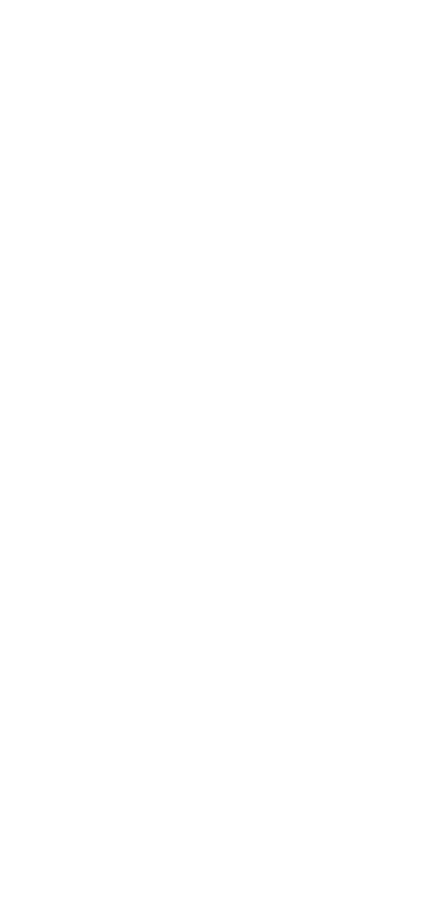
\includegraphics[height=0.3\textheight]{./Img/Experiment13_scheme.pdf}
	}}
}
\caption{Scheme of the simulated room}
\label{roomDimFig}
\end{figure}

\autoref{gainAverDifReflectCoef} shows the average gain histogram for different values of $\reflectCoef$. When it goes above $0.2$, the average gain reaches levels above $-10 \si{dB}$.

\begin{shownto}{private,publicGlobal}
\begin{figure}[h]
	\centering
	\begin{subfigure}[b]{0.45\textwidth}
		\centering
		\includegraphics[width=\columnwidth]{../TFM/Img/Experiment13_globalAttenReflCoef_0.eps}
		\caption{$\reflectCoef = 0$}
	\end{subfigure}
	\begin{subfigure}[b]{0.45\textwidth}
		\centering
		\includegraphics[width=\columnwidth]{../TFM/Img/Experiment13_globalAttenReflCoef_10.eps}
		\caption{$\reflectCoef = 0.1$}
	\end{subfigure}
	\begin{subfigure}[b]{0.45\textwidth}
		\centering
		\includegraphics[width=\columnwidth]{../TFM/Img/Experiment13_globalAttenReflCoef_20.eps}
		\caption{$\reflectCoef = 0.2$}
	\end{subfigure}
	\begin{subfigure}[b]{0.45\textwidth}
		\centering
		\includegraphics[width=\columnwidth]{../TFM/Img/Experiment13_globalAttenReflCoef_50.eps}
		\caption{$\reflectCoef = 0.5$}
	\end{subfigure}
	
	\caption{Global attenuation for different reflection coefficients $\reflectCoef$}
	\label{globAttenDifReflectCoef}
\end{figure}
\end{shownto}
\begin{figure}[h]
	\centering
	\begin{subfigure}[b]{0.45\textwidth}
		\centering
		\includegraphics[width=\columnwidth]{../TFM/Img/Experiment13_gainAverReflCoef_0.eps}
		\caption{$\reflectCoef = 0$}
	\end{subfigure}
	\begin{subfigure}[b]{0.45\textwidth}
		\centering
		\includegraphics[width=\columnwidth]{../TFM/Img/Experiment13_gainAverReflCoef_10.eps}
		\caption{$\reflectCoef = 0.1$}
	\end{subfigure}
	\begin{subfigure}[b]{0.45\textwidth}
		\centering
		\includegraphics[width=\columnwidth]{../TFM/Img/Experiment13_gainAverReflCoef_20.eps}
		\caption{$\reflectCoef = 0.2$}
	\end{subfigure}
	\begin{subfigure}[b]{0.45\textwidth}
		\centering
		\includegraphics[width=\columnwidth]{../TFM/Img/Experiment13_gainAverReflCoef_50.eps}
		\caption{$\reflectCoef = 0.5$}
	\end{subfigure}
	
	\caption{Average gain for different reflection coefficients $\reflectCoef$}
	\label{gainAverDifReflectCoef}
\end{figure}

\subsection{GTAC listening room}
The real impulse responses in the listening room are available in the research group website \cite{GTACroom}. They were measured with high precision for a rectangular grid of points of size $24$x$15$ separated a distance of $20\si{cm}$ between adjacent nodes \cite{Czy2011}. We could use those responses in calculations instead of the simulated ones. However, we found the limitation that
this measures were done only for the loudspeaker array, but not for loudspeakers outside the array in arbitrary positions. So, responses for potential noise sources are not available.

Nonetheless, there is an approach that can help us estimate what the performance in the real set up would be. We have seen that the existence of reflective surfaces worsens performance. The impulse response $h(t)$ from a source to a measuring point does not follow any more the ideal monopole free-space propagation equation in which the whole WFS theory is based.

In the time domain, the propagation in free-space conditions of a signal $\signal[ns][time](t)$ emitted by a monopole source to a given measure point separated a distance $d$, consists just of a delay equal to the time it takes to the signal to arrive at the measure point ($\tau = d/c$, where $c$ is the speed of sound) and an amplitude reduction proportional to the distance between the source and the measure point ($1/d$):
\begin{equation}
\Field[noValue][time](t) = \signal[ns][time](t) \ast h(t) = \signal[ns][time](t) \ast \frac{1}{d}\delta(t - \tau).
\end{equation}

In the frequency domain, this translates to
\begin{equation}
\Field[noValue][frequency](f) = \signal[ns][frequency](f) \ast H(f,d) = \signal[ns][frequency](f) \ast \frac{e^{-j\frac{2\pi f}{c}d}}{d}.
\end{equation}

A way of visualizing the deterioration is comparing the magnitude of the ideal response for a given distance, with the magnitude of the actual one. In \autoref{acPathRespRealCompDots} the ideal response is represented for $450 \si{Hz}$ by a line and the real one is represented with dots, where each dot represents a pair loudspeaker-measure point ($96$ loudspeakers, $360$ measure points, $96\cdot 360 = 34560$ dots). The $x$ value is the distance between source and measure point, and the $y$ value is the magnitude of the frequency response $\abs{H}$. A clearer way of visualizing it is a composed histogram as the ones used for the gain (\autoref{acPathRespRealCompHist}). 
Each coloured rectangle is delimited horizontally by two distance values ($x$ axis), and vertically by two magnitude values ($y$ axis). The colour represents the proportion of points that lie in that distance and magnitude interval with respect to the total amount of points for that given distance interval. In other words, each column is an independent probability histogram.

\begin{figure}[h]
	\centering
	\begin{subfigure}[b]{0.45\textwidth}
		\centering
		\includegraphics[width=\columnwidth]{../TFM/Img/Experiment13_AmpByDist_450HzDots.eps}
		\caption{}
		\label{acPathRespRealCompDots}
	\end{subfigure}
	\begin{subfigure}[b]{0.45\textwidth}
		\centering
		\includegraphics[width=\columnwidth]{../TFM/Img/Experiment13_AmpByDist_450HzHist.eps}
		\caption{}
		\label{acPathRespRealCompHist}
	\end{subfigure}
	\caption{Relation of frequency response and distance from source and receiver. Measured responses in the listening room.}
	\label{acPathRespRealComp}
\end{figure}

The difference is evident. Ideally, all dots (or all coloured rectangles) would lie on the line, but they don't. And the further away they are from the source, the more scattered they appear. But, how would this affect performance? We can make a rough estimate by comparing it with the deterioration produced in simulated scenarios. \autoref{acPathRespSimulComp} uses the same type of representation, but in this case, the impulse responses have not been measured in the real set up, but calculated with the Room Impulse Response generator using the listening room dimensions. A visual comparison over different values of the reflection coefficient $\reflectCoef$, suggests that the one that generates a most similar scenario to \autoref{acPathRespRealCompHist} is around $\reflectCoef = 0.8$ (magnitude values have been normaized). The average gain histogram simulated with that value, for the noise source configuration already used in previous subsection (\autoref{roomDimFig}) is shown in \autoref{gainAverSimilarReflectCoef}. As we can see, in most of the cases the average gain is even positive. This suggests that the possibility of performing noise cancellation with WFS techniques is very unlikely.

\begin{figure}[h]
	\centering
	\includegraphics[width=0.5\columnwidth]{../TFM/Img/Experiment13_RIRMagnDist08.eps}
	\caption{Relation of frequency response and distance from source and receiver. Simulated responses for $\reflectCoef = 0.8$.}
	\label{acPathRespSimulComp}
\end{figure}

\begin{figure}[h]
	\centering
	\includegraphics[width=0.5\columnwidth]{../TFM/Img/Experiment13_gainAverReflCoefSimil_80.eps}
	\caption{Average gain for $\reflectCoef = 0.8$.}
	\label{gainAverSimilarReflectCoef}
\end{figure}

\section{Truncation and lower cut-off frequency} % Experiment10.m
There is a remarkable phenomenon that can be observed through all simulations. If we take a look at any of the previously shown attenuation histograms, we will see that from approximately $200\si{Hz}$ down, the performance gets poorer as the frequency decreases. It is as if the system had a lower cut-off frequency of $200\si{Hz}$ below which it doesn't work properly (\autoref{lowCutOffFreqExample}). That transition region is there due to the fact that in practice, the line of secondary sources (the loudspeaker array) has a finite length, in other words, it is truncated. In order to explain this, it is convenient to recall some of the theoretical expressions of WFS.

\begin{figure}[h]
\centering
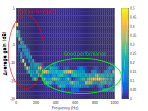
\includegraphics[width=0.5\columnwidth]{../TFM/Img/LowCutoffFrequencyDegradationExample.pdf}
\caption{Example of performance degradation for low frequencies}
\label{lowCutOffFreqExample}
\end{figure}

As we've already seen, the field created by a monopole source (primary source) located at $\PosTheo[primarySource]$ at a receiving point $\PosTheo$ is:
\begin{equation}
\Field[primarySource](\PosTheo) = \CoefTheo[primarySource](f)  \frac{e^{-jk\norm{\PosTheo - \PosTheo[primarySource]}}}{\norm{\PosTheo - \PosTheo[primarySource]}},
\end{equation}
where $f$ is the frequency, $\CoefTheo[primarySource](f)$ is the feeding coefficient to the source, and $k = \frac{2\pi}{\lambda}$ is the propagation constant.

Rayleigh I 2.5D integral allows to replicate the field by an infinite line distribution of monopole sources (secondary sources), given the condition that all points where the field is replicated, as well as the primary source location and the secondary source line distribution ($\sectionTheo$), are all on the same plane, and that the secondary source line separates the reconstructed field region from the primary source. The expression is:
\begin{equation}
\begin{aligned}
\Field(\PosTheo) &= \int_{\sectionTheo} \CoefTheo[section][monopole][rayleigh](\PosTheo[section], \PosTheo) \frac{e^{-jk\distLinePoint}}{\distLinePoint} \mathrm{d}\PosTheo[section],\\
\CoefTheo[section][monopole][rayleigh](\PosTheo[section]) &= \CoefTheo[primarySource] \cos\normPrimaryPropAngleSection \frac{e^{-jk\distLinePrimSource}}{\sqrt{\distLinePrimSource}} \sqrt{\frac{jk}{2\pi}} \sqrt{\frac{d}{d + d_{\PosTheoSubInd[primarySource]}}},
\end{aligned}
\end{equation}
where $Q(\PosTheo[section], \PosTheo)$ is the feeding of the differential secondary monopole source located at $\PosTheo[section]$, $\distLinePrimSource = \norm{\PosTheo[section] - \PosTheo[primarySource]}$ is the distance from the primary source to the secondary source and $\distLinePoint = \norm{\PosTheo[section] - \PosTheo}$ is the distance from the secondary source to the reconstruction point and $d_{\PosTheoSubInd[primarySource]}$ is the distance between the primary source and the secondary source line. It is valid for values of $k\distLinePrimSource >> 1$. The field is replicated with correct amplitude over a line parallel to the secondary source line and separated a distance $d$.

One of the reasons why Rayleigh I 2.5D integral is still far from practical applications is that the line distribution of monopoles $\sectionTheo$ has an infinite longitude, which is of course unrealistic. At some point the line has to be truncated, and hence, the accuracy of the reconstructed field will be affected.

In order to study this limitation, we can look at a simple scenario where a line of secondary sources $\sectionTheoLength$ meters long is located at the x axis from from $-\sectionTheoLength/2$ to $\sectionTheoLength/2$, a primary source is located on the negative y axis at $\PosTheo[primarySource] = [0, -d_{\PosTheoSubInd[primarySource]}, 0]$ and the receiving point on the positive y axis at $\PosTheo = [0, d, 0]$ (\autoref{truncationScheme}). Depending on those four parameters, three distances ($\sectionTheoLength$, $d_{\PosTheoSubInd[primarySource]}$ and $d$) plus the frequency $f$, the accuracy of the synthesized field will vary.

\begin{figure}[h]
	\centering
	\def\svgwidth{0.5\columnwidth}
	\graphicspath{{../TFM/Img/}}
	\input{../TFM/Img/Experiment10_truncationScheme.pdf_tex}
	\caption{Scheme of truncation scenario}
	\label{truncationScheme}
\end{figure}

In this scenario, the reconstructed field at point $\PosTheo$ is:
\begin{equation}
\Field(\PosTheo) = \int_{-\sectionTheoLength/2}^{\sectionTheoLength/2} \CoefTheo[section][monopole][rayleigh](\PosTheo[section][x], \PosTheo) \frac{e^{-jk\distLinePoint}}{\distLinePoint} \mathrm{d}\PosTheo[section][x],
\label{Rayleigh2_5DTruncatedIntegral}
\end{equation}
where $\distLinePrimSource = \norm{\PosTheo[section] - \PosTheo[primarySource]} = (d_{\PosTheoSubInd[primarySource]}^2 + \PosTheo[section][x]^2)^{1/2}$ is the distance from the primary source to the secondary source, $\distLinePoint = \norm{\PosTheo[section] - \PosTheo} = (d^2 + \PosTheo[section][x]^2)^{1/2}$ is the distance from the secondary source to the reconstruction point and $\cos\normPrimaryPropAngleSection = d_{\PosTheoSubInd[primarySource]}/\distLinePrimSource$ is the cosine of the angle of incidence.

A useful measure that facilitate the evaluation of the accuracy is the relative field $\Field_\mathit{rel}(\PosTheo)$, this is, the resulting field divided by the ideal one produced by the primary source.
\begin{equation}
	\Field_\mathit{rel}(\PosTheo) = \frac{\Field(\PosTheo)}{\Field[primarySource](\PosTheo)}.
\end{equation}
The closer $\Field_\mathit{rel}$ is to $0\si{dB}$ the better the accuracy. The starting point will be a very simple case, and then we will add some complexity.

\begin{shownto}{private}
This measure depend on the spatial parameters of the scenario (position of primary source $\PosTheo[primarySource]$, shape and location of the second source line distribution $\sectionTheo$, and location of the receiving point $\PosTheo$) and the wavelength $\lambda$. However, if we scale all parameters by a factor $C$ ($\PosTheo[primarySource]^{(s)} = C \PosTheo[primarySource]$, $\PosTheo^{(s)} = C\PosTheo$, $\PosTheo[section]^{(s)} = C\PosTheo[section]$, $\lambda^{(s)} = C\lambda$) and recalculate the signal of each secondary source, the relative field will be exactly the same due to the properties of the integral. This fact is useful because allows to, for example, express all distances in wavelengths ($d^{(s)} = d/\lambda$, $d_{\PosTheoSubInd[primarySource]}^{(s)} = d_{\PosTheoSubInd[primarySource]}/\lambda$, $L^{(s)} = L/\lambda$) and fixate the wavelength to $1$ ($\lambda = 1$), reducing the number of variables from four to three.
\end{shownto}

\subsection{Ideal case: $\sectionTheoLength=\infty$}
First, we consider an array of infinite length $\sectionTheoLength=\infty$.
% where each monopole secondary source transmits a signal $Q_\mathit{perfect}$:
%\begin{equation}
%Q_\mathit{perfect}(\PosTheo[section], \PosTheo) = \cos\normPrimaryPropAngleSection \frac{e^{-jk\distLinePrimSource}}{\sqrt{\distLinePrimSource}} \left(\sqrt{\frac{j k}{2\pi}} + \frac{1}{\distLinePrimSource \sqrt{j 2 \pi k}}\right) \sqrt{\frac{\distLinePoint}{\distLinePrimSource + \distLinePoint}}
%\end{equation}
Theoretically, any inexactitude must necessarily be produced by the application of the stationary point method in the dimensionality reduction from a plane to a line, and to the assumption that the primary source is in the far field $k\distLinePrimSource >> 1$ (\autoref{KirchoffDimReduction}).

In numerical calculation of the integral in Matlab (\autoref{TruncIdealRecFarPSclose}) shows that when $d_{\PosTheoSubInd[primarySource]}$ gets smaller, the reconstructed field deteriorates, and so WFS is actually not useful under such conditions. A similar behaviour but much less severe is found when the primary source is in the far field but the receiving point is very near the secondary source line (\autoref{TruncIdealPSFarRecClose}).
\begin{figure}[h]
	\centering
	\begin{subfigure}[b]{0.49\textwidth}
		\centering
		\includegraphics[width=0.9\textwidth]{Img/Experiment10_TruncationIdealCaseA.eps}
		\caption{$d/\lambda \gg 1$}
		\label{TruncIdealRecFarPSclose}
	\end{subfigure}
	\begin{subfigure}[b]{0.49\textwidth}
		\centering
		\includegraphics[width=0.9\textwidth]{Img/Experiment10_TruncationIdealCaseB.eps}
		\caption{$d_{\PosTheoSubInd[primarySource]}/\lambda \gg 1$}
		\label{TruncIdealPSFarRecClose}
	\end{subfigure}
	\caption{Magnitude and phase of the relative field for an infinite line array $\sectionTheoLength = \infty$}
\end{figure}
In conclusion, as long as both the primary source and the receiving point are not too close to the secondary source line, the precision will not be too distorted.

\subsection{Primary source in the infinite}
Let's take the case where the primary source is far: $d_{\PosTheoSubInd[primarySource]} \gg 1$. Then,
\begin{gather*}
	\cos\normPrimaryPropAngleSection \approx 1 \\ \distLinePrimSource \approx d \\ \sqrt{\frac{d}{d_{\PosTheoSubInd[primarySource]} + d}} \approx \sqrt{\frac{d}{d_{\PosTheoSubInd[primarySource]}}},
\end{gather*}
for all the segment $\PosTheo[section][x] \in [-\sectionTheoLength/2, \sectionTheoLength/2]$, so \autoref{Rayleigh2_5DTruncatedIntegral} simplifies to:
\begin{multline}
	P(\PosTheo) = \int_{-\sectionTheoLength/2}^{\sectionTheoLength/2} Q(x_{\PosTheoSubInd[section]}, \PosTheo) \frac{e^{-jk\distLinePoint}}{\distLinePoint} \mathrm{d}\PosTheo[section][x] =\\
	= \left\{Q(x_{\PosTheoSubInd[section]}, \PosTheo) =  \frac{e^{-jkd_{\PosTheoSubInd[primarySource]}}}{\sqrt{d_{\PosTheoSubInd[primarySource]}}} \sqrt{\frac{j k}{2\pi}} \sqrt{\frac{d}{d_{\PosTheoSubInd[primarySource]}}}\right\} = \\
	= \frac{e^{-jkd_{\PosTheoSubInd[primarySource]}}}{\sqrt{d_{\PosTheoSubInd[primarySource]}}} \sqrt{\frac{j k}{2\pi}} \sqrt{\frac{d}{d_{\PosTheoSubInd[primarySource]}}} \int_{-\sectionTheoLength/2}^{\sectionTheoLength/2} \frac{e^{-jk\distLinePoint}}{\distLinePoint} \mathrm{d}\PosTheo[section][x].
	\label{truncDeductionI}
\end{multline}

The integral is actually the field generated by a linear source. When we are dealing with an infinite line source ($\sectionTheoLength \to \infty$), the exact solution is a scaled version of the zero-th order of the Hankel function of second type. Nonetheless it approximates very well to another much more useful expression:
\begin{equation}
\int_{-\infty}^{\infty} \frac{e^{-jk\distLinePoint}}{\distLinePoint} \mathrm{d}x_{\PosTheoSubInd[section]} = -\pi j \mathrm{H_0^{(2)}(k d)} \approx \frac{e^{-jkd}}{\sqrt{kd}}\sqrt{\frac{2\pi}{j}}.
\label{fieldLinearSource}
\end{equation}

Substituting \autoref{fieldLinearSource} in \autoref{truncDeductionI}:
\begin{equation}
P(\PosTheo) \approx \frac{e^{-jkd_{\PosTheoSubInd[primarySource]}}}{\sqrt{d_{\PosTheoSubInd[primarySource]}}} \sqrt{\frac{j k}{2\pi}} \sqrt{\frac{d}{d_{\PosTheoSubInd[primarySource]}}} \frac{e^{-jkd}}{\sqrt{kd}}\sqrt{\frac{2\pi}{j}} = \frac{e^{-jk(d_{\PosTheoSubInd[primarySource]} + d)}}{d_{\PosTheoSubInd[primarySource]}} \approx \frac{e^{-jk(d_{\PosTheoSubInd[primarySource]} + d)}}{d_{\PosTheoSubInd[primarySource]} + d} = P_{\PosTheoSubInd[primarySource]}(\PosTheo).
\end{equation}

So, when $\sectionTheoLength \to \infty$, the synthesized field is the same as the field from the primary source, as stated by WFS theory. What happens when the length of the secondary source line gets shorter? It all comes dowm to the integral:
\begin{equation}
I(\lambda/\sectionTheoLength, d/\sectionTheoLength) = \int_{-\sectionTheoLength/2}^{\sectionTheoLength/2} \frac{e^{-jk\distLinePoint}}{\distLinePoint} \mathrm{d}\PosTheo[section][x] = \int_{-1/2}^{1/2} \frac{e^{-j\frac{2\pi}{\lambda/\sectionTheoLength}\sqrt{(d/\sectionTheoLength)^2 + \PosTheo[section][x]^2}}}{\sqrt{(d/\sectionTheoLength)^2 + \PosTheo[section][x]^2}} \mathrm{d}\PosTheo[section][x].
\label{lineSourceIntegralLfinite}
\end{equation}

\autoref{lineSourceIntegral} shows an example of how the integral evolves when increasing $\sectionTheoLength$. As we see, the magnitude and the phase oscillate and converges towards the value in \autoref{fieldLinearSource} when $\sectionTheoLength$ increases. It is pretty obvious that there is a transition period where $\sectionTheoLength$ is too small to produce accurate enough results.

\begin{figure}[h]
	\centering
	\includegraphics[width=0.4\textwidth]{Img/lineSourceIntegral.eps}
	\caption{Field generated by a linear source of length $L$ ($d = 10$, $k = 1$)}
	\label{lineSourceIntegral}
\end{figure}

As we've seen in \autoref{lineSourceIntegralLfinite}, $I$ depends actually just on $d/\sectionTheoLength$ and $\sectionTheoLength/\lambda$. In \autoref{lineSourceIntegralNorm} we've represented the value of $\sectionTheoLength/\lambda$ where the phase (and also the magnitude) starts to converge.

\begin{figure}[h]
	\centering
	\includegraphics[width=0.4\textwidth]{Img/LnormThreshold.eps}
	\caption{Minimum value of $\sectionTheoLength/\lambda$ where the value of $I$ (\autoref{lineSourceIntegralLfinite}) starts to converge}
	\label{lineSourceIntegralNorm}
\end{figure}

All this means that there is a lower cutoff frequency below which WFS is not useful. For example, \autoref{linseSourceIntegralGTAC} shows the cutoff frequency for a linear array of length $\sectionTheoLength = 0.18\cdot23 = 4.14\si{m}$, as one of the sides of the loudspeaker array in the GTAC listening room.
\begin{figure}[h]
	\centering
	\includegraphics[width=0.4\textwidth]{Img/freqThresholdGTAC.eps}
	\caption[Cutoff frequency for a linear array whose length is $\sectionTheoLength = 0.18\cdot23$]{Cutoff frequency for a linear array whose length is $\sectionTheoLength = 0.18\cdot23$, as two of the sides of the loudspeaker array in the GTAC listening room}
	\label{linseSourceIntegralGTAC}
\end{figure}

It's worth noticing that this analysis is done with a geometrically very simple scenario where the primary source is in the infinite, the receiving point is centred with respect to the secondary source line, we don't use complicated geometries as octagons, etc. The more variations we add, the more complex the results are. However, given what we observed in the simulations of the GTAC scenario, the existence of a lower cut-off frequency seems to be maintained even in those more complicated cases.

A deeper theoretical analysis of the truncation artefacts can be found in \cite[Section 4.3]{Start1997}, where various analytical approximations are proposed. Some techniques, as tapering, are proposed to reduce the effects of truncation, although they have only shown to work in mid and high frequencies.

\begin{shownto}{private}
\section{Sampling frequency influence}
\end{shownto}